\documentclass[usenames,dvipsnames,aspectratio=169]{beamer}

\usepackage[utf8]{inputenc}
\usepackage[T1]{fontenc}
\usepackage[magyar]{babel}
\usepackage{indentfirst}
\usepackage{graphicx}
\usepackage{listingsutf8}
\usepackage{textcomp}
\usepackage{eurosym}
\usepackage{mathtools}
\lstset{literate=
  {á}{{\'a}}1 {é}{{\'e}}1 {í}{{\'i}}1 {ó}{{\'o}}1 {ú}{{\'u}}1
  {Á}{{\'A}}1 {É}{{\'E}}1 {Í}{{\'I}}1 {Ó}{{\'O}}1 {Ú}{{\'U}}1
  {à}{{\`a}}1 {è}{{\`e}}1 {ì}{{\`i}}1 {ò}{{\`o}}1 {ù}{{\`u}}1
  {À}{{\`A}}1 {È}{{\'E}}1 {Ì}{{\`I}}1 {Ò}{{\`O}}1 {Ù}{{\`U}}1
  {ä}{{\"a}}1 {ë}{{\"e}}1 {ï}{{\"i}}1 {ö}{{\"o}}1 {ü}{{\"u}}1
  {Ä}{{\"A}}1 {Ë}{{\"E}}1 {Ï}{{\"I}}1 {Ö}{{\"O}}1 {Ü}{{\"U}}1
  {â}{{\^a}}1 {ê}{{\^e}}1 {î}{{\^i}}1 {ô}{{\^o}}1 {û}{{\^u}}1
  {Â}{{\^A}}1 {Ê}{{\^E}}1 {Î}{{\^I}}1 {Ô}{{\^O}}1 {Û}{{\^U}}1
  {œ}{{\oe}}1 {Œ}{{\OE}}1 {æ}{{\ae}}1 {Æ}{{\AE}}1 {ß}{{\ss}}1
  {ç}{{\c c}}1 {Ç}{{\c C}}1 {ø}{{\o}}1 {å}{{\r a}}1 {Å}{{\r A}}1
  {€}{{\EUR}}1 {£}{{\pounds}}1 {ő}{{\H{o}}}1 {ű}{{\H{u}}}1
}
\lstdefinestyle{HTML}{
  language=HTML,
  breaklines=true,
  postbreak=\mbox{\textcolor{red}{$\hookrightarrow$}\space},
  stringstyle=\ttfamily,
  inputencoding=utf8,
  morekeywords={header, time, nav, main, article, section, aside, role, 
    footer, details, open, summary, srcdoc, list, datalist, placeholder, 
    pattern, required, min, max, step, enctype, formaction, formmethod, 
    formnovalidate, formtarget, output}
}
\usepackage{hyperref}
\usepackage{attachfile}
\usepackage{multirow}
% Navigációs pöttyök hozzáadása subsection nélküli fejezetekhez
\usepackage{remreset}
\makeatletter
\@removefromreset{subsection}{section}
\makeatother
\setcounter{subsection}{1}
%%%%%
\attachfilesetup{color={1.0 0.6 0.0},author={HFM},description={Kattintson duplán a minta %
megtekintéséhez!},icon=Paperclip}
\definecolor{kiemelesszin}{rgb}{0.6,0.0,0.0}
\definecolor{kiemelesszinZ}{rgb}{0.0,0.6,0.0}
\definecolor{kiemelesszinN}{RGB}{196,127,0}
\definecolor{hivatkozasszin}{rgb}{0.0,0.0,0.75}
\newcommand{\kiemel}[1]{{\color{kiemelesszin}#1}}
\newcommand{\kiemelZ}[1]{{\color{kiemelesszinZ}#1}}
\newcommand{\kiemelN}[1]{{\color{kiemelesszinN}#1}}
\newcommand{\hiv}[1]{{\color{hivatkozasszin}#1}}
\frenchspacing
\usetheme[compress]{Berlin}

\title[Web technológiák - HTML]{Web-technológia}
\subtitle{HTML5, II. rész}
\author{Dr. Hatwágner F. Miklós}
\institute{Széchenyi István Egyetem, Győr}
\date{\hiv{\href{https://github.com/wajzy/GKxB\_INTM049.git}{https://github.com/wajzy/GKxB\_INTM049.git}}\\ \today}

\begin{document}

%1
\begin{frame}[plain]
  \titlepage
\end{frame}

\section{HTML5}

\subsection{Űrlapok}

%86
\begin{frame}
  Vastag kliens alkalmazásokhoz hasonlóan adatok gyűjthetőek űrlapokkal, amiket 
  \begin{itemize}
    \item feldolgoztathatunk a szerver oldalon (most ez lesz), vagy
    \item JavaScript programmal a kliensen.
  \end{itemize}
  Űrlap vezérlők a \texttt{<form>} elembe ágyazva használhatók. Legfontosabb attribútumai:
  \begin{description}[m]
    \item[\texttt{action}] \hfill \\ A szerver oldali feldolgozó script URL-je
    \item[\texttt{target}] \hfill \\ Hova töltse a szerver válaszát 
    (\texttt{\_blank}, \texttt{\_self} (alapért.), \texttt{\_parent}, \dots)
    \item[\texttt{novalidate}] \hfill \\ Ne végezzen input 
    ellenőrzést a böngésző
    \item[\texttt{autocomplete}] \hfill \\ Korábban megadottak alapján 
    kiegészíti az adatokat (\texttt{on} (alapért.), \texttt{off})
  \end{description}
\end{frame}

%87
\begin{frame}
  \begin{description}[m]
    \item[\texttt{method}] \hfill \\ Adattovábbítási módszer:
    \begin{description}[m]
      \item[\texttt{get}] \hfill \\ Alapértelmezett. URL lekérdező 
      karakterláncában továbbítja az adatokat.
      \begin{itemize}
        \item Az URL betehető a könyvjelzők közé, és
        \item a böngészőben is könnyen szerkeszthető
      \end{itemize}
      \item[\texttt{post}] \hfill \\ HTTP tranzakcióként továbbít.
      \begin{itemize}
        \item Nincsenek méretkorlátok (URL hossza korlátozott, 
        $\approx$ 2000 karakter)
        \item Fájlok csak így továbbíthatók
        \item A böngészőben nem látszik, de ettől még \kiemel{nyílt 
        szöveg}ként továbbítják a hálózaton!
      \end{itemize}
    \end{description}
  \end{description}
\end{frame}

%88
\begin{frame}
  \begin{description}[m]
    \item[\texttt{enctype}] (type of encoding) \hfill \\ Meghatározza 
    a küldött adatok kódolását. Kötelező megadni, ha a \texttt{method} 
    attr. értéke \texttt{post}. Lehetséges értékek:
    \begin{description}[m]
      \item[\texttt{application/x-www-form-urlencoded}] \hfill \\ 
      Alapértelmezett. Minden szóközt és speciális karaktert 
      helyettesít.
      \item[\texttt{multipart/form-data}] \hfill \\ Fájlok küldésekor 
      kell használni.
      \item[\texttt{\texttt{text/plain}}] \hfill \\ Csak a szóközöket 
      helyettesíti.
    \end{description}
  \end{description}
\end{frame}

%89
\begin{frame}
  A legtöbb vezérlő az \texttt{<input>} elemmel hozható létre, pl. 
  egy számbeviteli mező néhány attribútuma, és hatása:
  \begin{description}[m]
    \footnotesize
    \item[\texttt{type}] \hfill \\ \texttt{number}, számbeviteli mező 
    létrehozása
    \item[\texttt{name}] \hfill \\ A szerver oldalon ez lesz az adat 
    \emph{kulcsa}
    \item[\texttt{min}] \hfill \\ A legkisebb bevihető érték
    \item[\texttt{max}] \hfill \\ A legnagyobb bevihető érték
    \item[\texttt{step}] \hfill \\ Ennyit változtatnak a 
    léptetőgombok/kurzurvezérlő nyilak az értéken, ennyi 
    többszöröseit lehet megadni, illetve ha 
    értéke \texttt{any}, akkor bármilyen racionális szám megadható
    \item[\texttt{required}] \hfill \\ A mező kitöltése kötelező
  \end{description}
\end{frame}

%90
\begin{frame}
  Űrlapbeküldő gomb: \texttt{<input>} elem
  \begin{itemize}
    \item \texttt{type="submit"}
    \item \texttt{value} attr. adja meg a gomb feliratát
  \end{itemize}
  \vfill
  Cimke létrehozása vezérlőhöz: \texttt{<label>} elemmel. A 
  cimkére kattintva a vezérlő is aktiválódik (pl. rádiógombnál 
  kiválasztás). Kapcsolat cimke és 
  vezérlő között:
  \begin{itemize}
    \item vezérlő a cimke belsejébe ágyazva
    \item a cimke \texttt{for} attribútumában megadható a vezérlő 
    \texttt{id}-je
  \end{itemize}
\end{frame}

%91
\begin{frame}
  Vezérlők logikai csoportosítása: \texttt{<fieldset>} elemmel\\
  Csoport feliratának megadása: \texttt{<legend>} elemben
  \vfill
  \begin{center}
    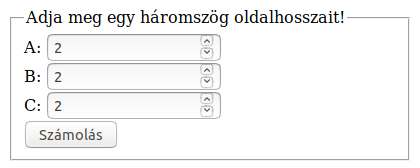
\includegraphics[width=.5\textwidth]{urlap1.png}
  \end{center}
\end{frame}

%92
\begin{frame}
  \begin{exampleblock}{\textattachfile{urlap1.html}{urlap1.html} 
  (\textattachfile{urlap1.php}{urlap1.php})}
    \footnotesize
    \lstinputlisting[style=HTML,linerange={8-20},numbers=left,firstnumber=8]{urlap1.html}
  \end{exampleblock}
\end{frame}


% blokkszintű és soron belüli elemek összefoglalója
% class és id attribútumok
% Data URI

\end{document}
